\documentclass[../Cours.tex]{subfiles}
\begin{document}

\chapitre{Probabilités}

\partie{Concept}

\definition{Une expérience est aléatoire si je ne peux pas déterminer à l'avance l'issue de l'évènement.}

\exemple{ << Lancer un dé à 6 faces >> est un évènement aléatoire, car je ne peux pas savoir à l'avance sur quoi va tomber le dé avant de le lancer.\\
Les issues de cette expérience sont $\Omega = {1;2;3;4;5;6}$.}

\definition{La probabilité d'un évènement est un nombre entre 0 et 1 qui permet de quantifier la possibilité que l'évènement se réalise.}

\partie{Approche qualitative}

\begin{center}
    \begin{tikzpicture}
        \node[rouge,text width=3.5cm] at (-6,0) {évènement impossible};
        \node[rouge,text width=3.5cm] at (-2,0) {évènement peu probable};
        \node[rouge,text width=3.5cm] at (2,0) {évènement probable};
        \node[rouge,text width=3.5cm] at (6,0) {évènement certain};
        \draw[dashed] (-4,1) -- (-4,-3);
        \draw[dashed] (0,1) -- (0,-3);
        \draw[dashed] (4,1) -- (4,-3);
        \draw[-latex] (-8,-1) -- (8,-1);
        \node[noir, text width=3.5cm] at (-6,-2) {lancer un dé et obtenir un 0};
        \node[noir, text width=3.5cm] at (-2,-1.5) {gagner au loto};
        \node[noir, text width=3.5cm] at (-2,-2.5) {avoir un 1 en lançant un dé};
        \node[noir, text width=3.5cm] at (2,-1.5) {perdre au loto};
        \node[noir, text width=3.5cm] at (2,-3) {avoir entre 2 et 6 en lançant un dé};
        \node[noir, text width=3.5cm] at (6,-2.5) {lancer un dé et avoir un nombre entre 1 et 6};
    \end{tikzpicture}
\end{center}    

\clearpage
\partie{Approche quantitative}

\propriete{La probabilité d'une issue est égale à $\dfrac{1}{\card({\Omega})}$,\\ $\card({\Omega})$ est le nombre d'issues au total.}

\begin{listedexemples}
    \item Pile ou face : $\Omega = \left\{ \mbox{"pile"} ; \mbox{"face"} \right\}$, $\card{(\Omega)} = 2$\\
    $p\left( \mbox{pile} \right) = \dfrac{1}{2}$
    \item Lancer de dé : $\Omega = \left\{ 1;2;3;4;5;6 \right\}, \card{(\Omega)} = 6 $\\
    $p\left( \mbox{avoir un 3} \right) = \dfrac{1}{6}$
    \item On choisit une lettre au hasard dans l'alphabet :\\
    $\Omega = \left\{ A; B; C; D; E; F; G; H; I; J; K; L; M; N; O; P; Q; R; S; T; U; V; W; X; Y; Z \right\}$\\
    $\card{(\Omega)} = 26$\\
    $p\left( \mbox{avoir un H} \right) = \dfrac{1}{26}$
\end{listedexemples}

\definition{Un évènement est un ensemble d'issues.}

\exemple{Pour l'expérience aléatoire << lancer un dé >> :\\
A = << obtenir un nombre pair >> $= \left\{ 2;4;6 \right\}$\\
B = << obtenir un nombre premier >> $= \left\{ 2;3;5 \right\} $}

\propriete{La probabilité d'un évènement A est égale à $\dfrac{\card{(A)}}{\card{(\Omega)}}$}

\exemple{Dans l'expérience aléatoire de lancer un dé, $\Omega = \left\{ 1;2;3;4;5;6 \right\}$.\\ 
L'évènement A = << obtenir un nombre pair >> $= \left\{ 2;4;6 \right\} \longrightarrow \card{(A)} = 3$\\
$p(A) = \dfrac{3}{6}$}

\clearpage
\EXERCICES
\begin{questions}
    \exercice Dans chacune des situations suivantes, dire s'il s'agit d'une expérience aléatoire ou non.
    \question On choisit au hasard un élastique à cheveux dans un panier qui en contient 2 bleus, 3 rouges, 4 verts et 1 orange.
    \question On verse un morceau de sucre dans une tasse remplie de café chaud.
    \question Pour départager deux personnes, on décide de faire un << pile ou face >>.
    
    \exercice Pour chacun des évènements suivants, donner l'ensemble des issues qui le compose. Préciser, le cas échéant, si l'évènement est certain ou impossible.
    \question On lance un dé classique (à 6 faces numérotées de 1 à 6, cubique, non truqué) et on s'intéresse au résultat du lancer du dé.
        \subquestion{Évènement A : << Obtenir un nombre inférieur à 4. >>}
        \subquestion{Évènement B : << Obtenir un nombre supérieur ou égal à 5. >>}
        \subquestion{Évènement C : << Obtenir un nombre égal à 7. >>}

    \question On tire une lettre au hasard dans l'alphabet français.
        \subquestion{Évènement D : << Obtenir une voyelle. >>}
        \subquestion{Évènement E : << Obtenir une consonne ou une voyelle. >>}

    \exercice On choisit au hasard, sans regarder, une des figures suivantes :
    \begin{center}
        \begin{tikzpicture}[scale=0.7]
            \draw (0,0) rectangle (10,6);
            \filldraw[rouge] (3,4) -- +({cos(60)},{sin(60)}) -- +(1,0) -- cycle;
            \filldraw[orange] (2,1) -- +({cos(60)},{sin(60)}) -- +(1,0) -- cycle;
            \filldraw[bleu] (8,3) -- +({cos(60)},{sin(60)}) -- +(1,0) -- cycle;
            \filldraw[vert] (1,4.5) rectangle +(1,1);
            \filldraw[rouge] (6,1) rectangle +(1,1);
            \filldraw[jaune] (7,4) rectangle +(1,1);
            \filldraw[bleu] (1.5,2.5) rectangle +(1,1);
            \filldraw[vert] (5,2) circle (0.6);
            \filldraw[vert] (6,4) circle (0.6);
            \filldraw[orange] (9,1) circle (0.6);
        \end{tikzpicture}
    \end{center}

    \question Si l'on s'intéresse uniquement à la couleur des figures, quelles sont les issues ?
    \question Citer toutes les issues constituant les évènements suivants :
        \subquestion{Évènement R : << La figure est rouge >>}
        \subquestion{Évènement C : << La figure est un carré >>}
    \question Les évènements ci-dessous sont-ils certains ? impossibles ?
        \subquestion{Évènement G : << La figure est une forme géométrique >>}
        \subquestion{Évènement N : << La figure est de couleur noire >>}
        \subquestion{Évènement D : << La figure est un disque >>}

    \exercice Un élève lance une pièce de \qty{2}{\EURO} huit fois de suite, et à chaque fois il a obtenu << pile >>. Qu'obtiendra-t-il au lancer suivant ?
        \subquestion{pile}
        \subquestion{face}
        \subquestion{on ne peut pas savoir}

    \exercice Un élève choisit un bonbon dans un sachet de bonbons colorés. Elle se demande quelle serait la probabilité d'avoir un bonbon rouge. Le nombre de bonbons par couleur est illustré par le diagramme en barres suivant :
    \begin{center}
        \begin{tikzpicture}[xscale=1.7, yscale=0.6]
            \draw (0,0) -- (8,0);
            \draw[-Latex] (0,0) -- (0,7);
            \foreach \y in {1,...,6} {
                \draw (-0.2,\y) node[anchor=east]{\y} -- (0,\y);
                \draw[noir!30!blanc] (0,\y) -- (8,\y); 
            };
            \foreach[count=\i] \c/\y in {rouge/6,orange/5,jaune/3,vert/3,bleu/2,rose/4,violet/2,marron/5} {
                \draw (\i,-0.2) -- (\i,0);
                \filldraw[\c] ({\i-0.6},0) rectangle ({\i-0.4}, \y);
                \node[below] at ({\i-0.5},0) {\c \vphantom{bljg}};
            };
            \node[anchor=west] at (0,7) {Nombre de bonbons};
        \end{tikzpicture}
    \end{center}

    \question La probabilité d'avoir un bonbon rouge est :
        \subreponse{\qty{6}{\%}}
        \subreponse{\qty{20}{\%}}
        \subreponse{$\dfrac{1}{5}$}
        \subreponse{$0{,}2$}

    \exercice Dans chaque cas, dire s'il s'agit d'une expérience aléatoire.
    \question Jouer au loto.
    \question Répondre à un QCM.
    \question Tirer au hasard une carte dans un jeu de 32 cartes.
    \question Tirer au hasard une boule dans un sac ne contenant que des boules noires.

    \exercice Yann tire au sort une lettre au hasard dans l'alphabet français. Pour chacun des évènements suivants, donner l'ensemble des issues qui le constitue.
    \question Évènement V : << La lettre est une voyelle >>
    \question Évènement P : << La lettre figure dans son prénom >>
    \question Évènement R : << La lettre figure deux fois dans son prénom. >>

    \exercice On tire au hasard une carte dans un jeu de 32 cartes.
    \question De quelles issues sont constituées les évènements suivants :
        \subquestion{Évènement A : << La carte est un roi >>}
        \subquestion{Évènement B : << La carte est un trèfle >>}
    \question Que peut-on dire de l'évènement << La carte est un 3 >> ?

    \exercice À un stand de fête foraine, on gagne un lot si on tire le chiffre 1. La joueur a le choix entre : lancer un dé dont le patron est ci-dessous à gauche, ou jouer à la roulette à droite.

    \begin{center}
        \begin{tikzpicture}
            \filldraw[vert!70!white] (0,0) rectangle (1,1) node[midway,white]{1};
            \filldraw[vert!70!white] (1,1) rectangle (2,2) node[midway,white]{1};
            \filldraw[vert!70!white] (1,-1) rectangle (2,0) node[midway,white]{1};
            \filldraw[vert!70!white] (3,0) rectangle (4,1) node[midway,white]{1};
            \filldraw[bleu!40!white] (1,0) rectangle (2,1) node[midway,white]{2};
            \filldraw[rouge!60!white] (2,0) rectangle (3,1) node[midway,white]{3};
            \draw (0,0) rectangle (4,1);
            \draw (1,-1) rectangle (2,2);
            \draw (3,0) -- (3,1);
        \end{tikzpicture} \hspace{2cm}
        \begin{tikzpicture}
            \tikzmath{ \r=1.6; }
            \filldraw[vert!70!white] (0,0) -- ({\r*cos(135)},{\r*sin(135)}) arc (135:315:\r) -- cycle;
            \filldraw[bleu!40!white] (0,0) -- ({\r*cos(135)},{\r*sin(135)}) arc (135:45:\r) -- cycle;
            \filldraw[rouge!60!white] (0,0) -- (\r,0) arc (0:-45:\r) -- cycle;
            \filldraw[vert!70!white] (0,0) -- (\r,0) arc (0:45:\r) -- cycle;
            \draw (0,0) circle (\r);
            \draw ({\r*cos(45},{\r*cos(45)}) -- ({\r*cos(225)},{\r*sin(225)});
            \draw ({\r*cos(-45)},{\r*sin(-45)}) -- ({\r*cos(135)},{\r*sin(135)});
            \draw (-\r,0) -- (\r,0);
            \draw (0,-\r) -- (0,\r);
            \foreach[count=\i from 0] \n in {1,2,2,1,1,1,1,3} {
                \node[white] at ({0.707*\r*cos((\i+0.5)*45)},{0.707*\r*sin((\i+0.5)*45)}) {\n};
            }
        \end{tikzpicture}
    \end{center}
    \question Que doit choisir le joueur pour avoir le plus de chances de gagner ?

    \clearpage
    \exercice On donne 12 jetons identiques, puis on les numérote comme ci-dessous et on les range dans une boîte opaque.

    \begin{center}
        \begin{tikzpicture}[scale=0.6]
            \foreach[count=\i from 0] \n in {1,3,4,1,5,2,2,5,1,1,3,5} {
                \filldraw[noir] ({3*mod(\i,6)},{-2.5*int(\i/6)}) circle (1);
                \filldraw[white] ({3*mod(\i,6)},{-2.5*int(\i/6)}) node[rouge]{\Large\bfseries\n} circle (0.7);
            }
        \end{tikzpicture}
    \end{center}

    On tire au sort un jeton dans la boîte.
    \question Définir à l'aide d'une phrase un évènement A dont les issues seraient $\left\{ 1;2;3 \right\}$.
    \question Définir à l'aide d'une phrase un évènement B dont les issues seraient $\left\{ 1;3;5 \right\}$.
    \question Justin affirme qu'il a plus de chances d'obtenir un nombre pair qu'un nombre impair. A-t-il raison ?

    \exercice Pour préparer la prochaine élection, un organisme de presse commande un sondage. Voici les résultats du sondage :
    \begin{center}
        \begin{tabularx}{0.5\linewidth}{|X|X|}\hline
            Nom du candidat & Nombre de votes \\ \hline
            Candidat A & 791 \\ \hline
            Candidat B & 204 \\ \hline
        \end{tabularx}
    \end{center}
    \question La probabilité qu'une personne répondant au sondage ait choisi le candidat A \\est environ égale à :
        \subreponse{0{,}4}
        \subreponse{0{,}63}
        \subreponse{0{,}8}

    \exercice Dans un magasin, des statistiques ont été effectuées à partir d'un grand nombre de données sur le temps d'attente en caisse :
    \begin{center}
        \begin{tabularx}{0.5\linewidth}{|X|X|}\hline 
            Durée d'attente & Fréquence \\\hline
            Moins de 5 minutes & $0,2$ \\\hline 
            Entre 5 et 10 minutes & $0,4$ \\\hline
            Entre 10 et 15 minutes & $0,38$ \\\hline 
            Plus de 15 minutes & $0,02$ \\\hline
        \end{tabularx}
    \end{center}

    Un client se présente en caisse.
    \question Déterminer la probabilité qu'il attende moins de 10 minutes. Exprimer cette probabilité sous forme décimale et sous forme de pourcentage.
    \question Quelle est la probabilité qu'il attende plus de 5 minutes ? Exprimer cette probabilité sous forme de fraction simplifiée.

    \exercice
    \begin{center}
        \begin{tikzpicture}
            \tikzmath{ \r=1.4; }
            \draw (0,0) circle (\r);
            \draw ({\r*cos(30)},{\r*sin(30)}) -- ({\r*cos(210)},{\r*sin(210)});
            \draw ({\r*cos(330)},{\r*sin(330)}) -- ({\r*cos(150)},{\r*sin(150)});
            \draw (0,\r) -- (0,-\r);
        \end{tikzpicture}
    \end{center}

    \question Colorier la roue ci-dessus pour qu'elle soit constituée de deux issues de même probabilité.
    \question Colorier la roue ci-dessus pour que toutes ses issues aient une probabilité de $\frac{1}{3}$.

    \clearpage
    \exercice Deux urnes contiennent des boules \emph{indiscernables} au toucher. On choisit une des deux urnes et on tire une boule au hasard. On gagne si la boule obtenue est rouge.
    \begin{itemize}
        \item Dans la première urne, il y a 35 boules rouges et 65 boules jaunes.
        \item Dans la deuxième urne, il y a 19 boules rouges et 31 boules jaunes.
    \end{itemize}
    \question Dans laquelle de ces deux urnes a-t-on le plus de chances de gagner ?

    \exercice Dans un lac artificiel carré, on a construit une île carrée, comme représentée dans la figure ci-dessous. Un canard se pose au hasard sur le lac.

    \begin{center}
        \begin{tikzpicture}
            \filldraw[bleu!30!cyan] (0,0) rectangle (6,6);
            \draw[noir!20!blanc] (0,0) grid (6,6);
            \filldraw[rouge,rotate around={45:(4,3)}] (4,3) rectangle +(1.414,1.414) node[midway,blanc]{\bfseries\Large île};
        \end{tikzpicture}
    \end{center}

    \question Calculer la probabilité que la canard se pose sur l'île.
    \question Exprimer cette probabilité sous forme de fraction simplifiée.

    \exercice Dans un jeu de cartes de 32 cartes classiques, Victor choisit au hasard une carte dans le paquet.
    \question Donner la liste de toutes les issues possibles ?
    \question Quel est le nombre d'issues possibles ?
    \question Quelle est la probabilité de tirer un valet de carreau ?
    \question Quelle est la probabilité de tirer une carte trèfle ?
    
    \exercice Une urne opaque contient trois boules rouges et deux boules bleues, indiscernables au toucher. Laure tire au hasard une boule dans l'urne.
    \question Quelle est la probabilité de tirer une boule rouge ?
    \question Quelle est la probabilité de tirer une boule bleue ?
    \question Donner les deux résultats précédents sous forme de pourcentage.
    
    \exercice Une roue est divisée en trois secteurs de couleurs différentes. Jérôme fait tourner la roue.
    
    \question Pourquoi peut-on dire que les trois couleurs ont autant de chances d'être obtenues ?
    \question Quelle est la probabilité d'obtenir une des trois couleurs ? Donner le résultat sous forme de fraction, de nombre décimal et de pourcentage.
    
    
    \begin{center}
        \begin{tikzpicture}[scale=1.4]
            \draw[fill=noir] (0,1) -- (0.1,1.2) -- (-0.1,1.2) -- cycle;
            \draw[rouge,fill=rouge] (0,0) -- (1,0) arc(0:120:1) -- cycle;
            \draw[bleu, fill=bleu] (0,0) -- (1,0) arc(0:-120:1) -- cycle;
            \draw[vert, fill=vert] (0,0) -- ({cos(120)},{sin(120)}) arc(120:240:1) -- cycle;
        \end{tikzpicture}
    \end{center}
    
    \exercice Sur les 6 faces d'un dé standard, on inscrit les lettres du mot TOUPIE.
    \question Quelles sont les issues de l'expérience ?
    \question Donner la probabilité de chacune des lettres possibles sous forme de fraction.
    
    \exercice On lance une pièce de monnaie. 
    \question Lancer la pièce 50 fois et noter le nombre de fois qu'on tombe sur pile et sur face.
    \question Quelle est la probabilité de tomber sur pile, de tomber sur face ?
    \question Est-ce cohérent avec ce que vous avez trouvé ?
    
    \exercice Dans un jeu de 32 cartes :
    \question Donner les issues de l'évènement A : << Avoir un as >>
    \question Donner les issues de l'évènement B : << Avoir un valet >>
    \question Donner les issues de l'évènement C : << Avoir une carte pique >>
    \question Donner les issues de l'évènement D : << Avoir une figure >>
    \question Pour chacun des évènements A, B, C et D, donner leur probabilité.
    
    \exercice 
    \question Construire le patron d'un dé à 6 faces.
    \question Lancer le dé 36 fois et noter les résultat, cela est-il cohérent ?

    \exercice Dans une urne, il y a 45 boules jaunes, 25 boules bleues, 30 boules rouges.
    \question Quelles sont les issues ?
    \question Quelle est la probabilité de tirer une boule rouge ?
    \question L'évènement A : << avoir une boule de couleur primaire (rouge, vert, bleu) >>. Calculer la probabilité de l'évènement A.

    \exercice Dans une urne, il y a 12 jetons bleu marine, 17 jetons rouge bordeaux et 22 jetons violet clair.
    \question Quelles sont les issues ?
    \question Calculer toutes les probabilités. Donner les résultats en pourcentage.

    \exercice
    \question Quelle est la probabilité que deux personnes aient le même anniversaire ?
    \question Quelle est la probabilité qu'un bébé soit un garçon sachant que le ratio garçon-fille est de 1004:1000.

\end{questions}

\clearpage
\CORRECTIONS
\begin{questions}
    \exercice 
    \question Puisqu'on choisit \textit{au hasard}, cela signifie que l'on ne pourra pas connaître à l'avance la couleur de l'élastique que l'on obtiendra. Il s'agit donc d'une expérience aléatoire dont l'univers est $\Omega = \left\{ \mbox{bleu, rouge, vert, orange} \right\}$.
    \question On peut savoir à l'avance que si l'on met un morceau de sucre dans du café, le sucre va se dissoudre dans le café. Il n'y a rien d'aléatoire là dedans.
    \question Un << pile ou face >> est une expérience aléatoire car, au moment de lancer la pièce, je ne peux pas savoir \textit{a priori} (à l'avance) si elle tombera sur pile ou sur face. C'est donc aléatoire et l'univers est $\Omega = \left\{ \mbox{pile, face} \right\}$.

    \exercice 
    \question 
        \subquestion Lorsque l'on lance un dé, pour << obtenir un nombre inférieur à 4 >>, les seules possibilités sont d'avoir un 1, un 2 ou un 3. Donc $A = \left\{ 1, 2, 3 \right\}$.
        \subquestion Lorsque l'on lance un dé, pour << obtenir un nombre supérieur ou égal à 5 >>, les seules possibilités sont d'avoir un 5 ou un 6. Donc $B = \left\{ 5, 6 \right\}$.
        \subquestion Lorsque l'on lance un dé, on ne peut pas << obtenir un nombre égal à 7 >> parce qu'un dé va de 0 à 6. Donc $C = \vide$, $C$ est \emph{impossible}.
    \question 
        \subquestion Dans l'alphabet français, il y a 6 voyelles. $D = \left\{ a, e, i, o, u, y \right\}$.
        \subquestion Dans l'alphabet français, il n'y a que des consonnes et des voyelles. Donc si l'évènement est << Obtenir une consonne ou une voyelle >>, alors cela peut correspondre à n'importe quelle lettre de l'alphabet. Il est \textit{certain} que si l'on tire au hasard une lettre de l'alphabet, on obtiendra une consonne ou une voyelle. $E = \Omega$.

    \exercice
    \question Les issues sont $\Omega = \left\{ \mbox{rouge, vert, bleu, jaune, orange} \right\}$.
    \question 
        \subquestion $R = \left\{ \mbox{triangle rouge, carré rouge} \right\}$
        \subquestion $C = \left\{ \mbox{carré vert, carré bleu, carré rouge, carré jaune }\right\}$
    \question 
        \subquestion Cette évènement est certain. En effet, quelque soit la figure que l'on aura tirée au hasard, ce sera forcément une forme géométrique. $G=\Omega$.
        \subquestion Aucune des figures n'est de couleur noire, donc tirer au hasard une figure noire est impossible. $N = \vide$.
        \subquestion Il est possible de tirer au hasard un disque, comme il est possible de tirer autre chose. Ici, l'évènement D n'est ni certain ni impossible.

    \exercice Même si on obtient huit fois de suite << pile >>, cela n'influence en rien les lancers suivants. Chaque lancer de pièce est \emph{indépendant} des autres. Ici, la réponse était donc << on ne peut pas savoir >>.

    \exercice Si on compte la totalité des bonbons en lisant le graphique, il y a $6+5+3+3+2+4+2+5=30$ bonbons, dont 6 bonbons rouges. On peut donc dire que la probabilité d'avoir un bonbon rouge est de $\frac{6}{30}$. \\
    Mais lorsque l'on fait le calcul, $\frac{6}{30} = \frac{6 \times 1}{6 \times 5} = \frac{1}{5}$.\\
    De plus, $\frac{1}{5} = 1 \div 5 = 0{,}2$.\\
    En outre, $0,2 = 0,2 \times 1 = 0,2 \times \frac{100}{100} = \frac{0,2 \times 100}{100} = \frac{20}{100} = 20~\%$.\\
    Il y avait donc trois réponses justes : \textbf{b)~c)~d)}.

    \exercice 
    \question Jouer au loto est une expérience \emph{aléatoire}, car on ne peut pas connaître à l'avance les numéros gagnants.
    \question Répondre à un QCM \emph{n'est pas aléatoire} car il est possible de connaître les réponses aux questions posées (c'est même le but d'un QCM).
    \question Tirer au hasard une carte dans un jeu de 32 cartes est bien \emph{aléatoire} ; la présence de l'expression << au hasard >> nous renseigne bien sur le fait que l'on peut tomber sur n'importe laquelle des 32 cartes sans savoir \emph{a priori} celle que l'on obtiendra.
    \question Bien que l'on utilise aussi l'expression << au hasard >>, ici elle n'est pas pertinente. En effet, dans le sac, il n'y a que des boules noires. Donc même si on en tire une au hasard, on sait d'avance que la boule obtenue sera noire, puisqu'il n'y a que ça.

    \exercice 
    \question $V = \left\{ a, e, i, o, u, y \right\}$
    \question $P = \left\{ y, a, n \right\}$
    \question $R = \left\{ n \right\}$

    \exercice 
    \question
        \subquestion $A = \left\{ \mbox{roi de pique, roi de trèfle, roi de coeur, roi de carreau} \right\}$
        \subquestion $B = \left\{ \mbox{as de trèfle, roi de trèfle, dame de trèfle, valet de trèfle, 10 de trèfle, 9 de trèfle, 8 de trèfle, 7 de trèfle} \right\}$
    \question Cet évènement est \emph{impossible} car il n'y a aucune carte << 3 >> dans le paquet.

    \exercice Si on choisit le dé, on a 4 chances sur 6 de gagner. Si on choisit la roulette, on a 5 chances sur 8 de gagner. La question est de savoir quel est le nombre le plus grand entre $\frac{4}{6}$ et $\frac{5}{8}$.\\

    Soit on passe par la forme décimale : $\frac{4}{6} = 0,666...$ et $\frac{5}{8} = 0,6$.\\
    Soit on remet tout au même dénominateur. La première fraction est sur 6, la deuxième est sur 8, on va donc tout mettre sur $6 \times 8 = 48$.\\

    \vspace{-5ex}\begin{align*}
        &\dfrac{4}{6} = \dfrac{4 \textcolor{rouge}{\times 8}}{6 \textcolor{rouge}{\times 8}} = \dfrac{32}{48} \\ 
        &\dfrac{5}{8} = \dfrac{5 \textcolor{rouge}{\times 6}}{8 \textcolor{rouge}{\times 6}} = \dfrac{30}{48}
    \end{align*}

    Quelque soit la méthode, on en conclut que $\frac{4}{6} > \frac{5}{8}$, ce qui signifie qu'on aura plus de chances de gagner avec le dé plutôt qu'avec la roulette.

    \exercice 
    \question L'évènement << avoir un nombre entre 1 et 3 >> correspond bien aux issues $\left\{ 1;2;3 \right\}$.
    \question L'évènement << avoir un nombre impair >> correspond bien aux issues $\left\{ 1;3;5 \right\}$.
    \question Sur les 12 jetons, il y en a 9 impairs et 3 pairs. Il n'y a donc pas la même probabilité d'avoir des pairs et des impairs.

    \exercice Pour calculer la probabilité qu'une personne ait choisi le candidat A, il faudrait calculer $\frac{791}{791+204}$, c'est-à-dire le nombre de personnes ayant choisi le candidat A divisé le nombre de personnes interrogées au total.\\
    On peut approximer le résultat $\frac{791}{791+204} \approx \frac{800}{1000} = 0,8$. Il fallait donc choisir la réponse \textbf{c)}.

    \clearpage
    \exercice 
    \question Attendre moins de 10 minutes correspond à la fois à << moins de 5 minutes >> et à << entre 5 et 10 minutes >>.\\
    On va noter :
    \begin{itemize}
        \item $p(t<10)$ la probabilité que le temps ($t$) d'attente soit inférieur à 10 minutes
        \item $p(t<5)$ la probabilité que le temps d'attente ($t$) soit inférieur à 5 minutes
        \item $p(5<t<10)$ la probabilité que le temps d'attente ($t$) soit entre 5 et 10 minutes
    \end{itemize} 
    Avec cette notation, on a : $p(t<10) = p(t<5) + p(5<t<10) = 0,2+0,4 = 0,6$.\\
    Donc la probabilité d'attendre moins de 10 minutes est de 0,6 = \qty{60}{\%}.
    \question Selon la même logique et la même notation : 
    $$ p(t>5) = p(5<t<10) + p(10<t<15) + p(t>15) = 0,4+0,38+0,02=0,8=\qty{80}{\%} = \frac{4}{5}$$

    \exercice
    \question S'il y a deux issues de même probabilité, et 6 secteurs à colorier, alors on aura 2 couleurs et chaque couleur devra être présente sur 3 secteurs.\\
    Voici 3 réponses possibles (il y en a plein d'autres) :
    \begin{center}
        \begin{tikzpicture}
            \tikzmath{ \r=1.4; }
            \foreach[count=\i from 0] \s in {vert,rouge,rouge,vert,rouge,vert} {
                \filldraw[\s] (0,0) -- ({\r*cos(60*(\i+0.5))},{\r*sin(60*(\i+0.5))}) arc({60*(\i+0.5)}:60*(\i+1.5):\r) -- cycle;
            };
            \draw (0,0) circle (\r);
            \draw ({\r*cos(30)},{\r*sin(30)}) -- ({\r*cos(210)},{\r*sin(210)});
            \draw ({\r*cos(330)},{\r*sin(330)}) -- ({\r*cos(150)},{\r*sin(150)});
            \draw (0,\r) -- (0,-\r);
        \end{tikzpicture}
        \begin{tikzpicture}
            \tikzmath{ \r=1.4; }
            \foreach[count=\i from 0] \s in {jaune,jaune,jaune,bleu,bleu,bleu} {
                \filldraw[\s] (0,0) -- ({\r*cos(60*(\i+0.5))},{\r*sin(60*(\i+0.5))}) arc({60*(\i+0.5)}:60*(\i+1.5):\r) -- cycle;
            };
            \draw (0,0) circle (\r);
            \draw ({\r*cos(30)},{\r*sin(30)}) -- ({\r*cos(210)},{\r*sin(210)});
            \draw ({\r*cos(330)},{\r*sin(330)}) -- ({\r*cos(150)},{\r*sin(150)});
            \draw (0,\r) -- (0,-\r);
        \end{tikzpicture}
        \begin{tikzpicture}
            \tikzmath{ \r=1.4; }
            \foreach[count=\i from 0] \s in {jaune,noir,jaune,noir,jaune,noir} {
                \filldraw[\s] (0,0) -- ({\r*cos(60*(\i+0.5))},{\r*sin(60*(\i+0.5))}) arc({60*(\i+0.5)}:60*(\i+1.5):\r) -- cycle;
            };
            \draw (0,0) circle (\r);
            \draw ({\r*cos(30)},{\r*sin(30)}) -- ({\r*cos(210)},{\r*sin(210)});
            \draw ({\r*cos(330)},{\r*sin(330)}) -- ({\r*cos(150)},{\r*sin(150)});
            \draw (0,\r) -- (0,-\r);
        \end{tikzpicture}
    \end{center}
    \question Si chaque issue a une probabilité de $\frac{1}{3}$, cela signifie qu'il y aura 3 issues, donc 3 couleurs. Puisqu'il y a 6 secteurs, il faut que chaque couleur ait deux secteurs.\\
    Voici 3 réponses possibles (il y en a plein d'autres) :
    \begin{center}
        \begin{tikzpicture}
            \tikzmath{ \r=1.4; }
            \foreach[count=\i from 0] \s in {jaune,rouge,vert,jaune,rouge,vert} {
                \filldraw[\s] (0,0) -- ({\r*cos(60*(\i+0.5))},{\r*sin(60*(\i+0.5))}) arc({60*(\i+0.5)}:60*(\i+1.5):\r) -- cycle;
            };
            \draw (0,0) circle (\r);
            \draw ({\r*cos(30)},{\r*sin(30)}) -- ({\r*cos(210)},{\r*sin(210)});
            \draw ({\r*cos(330)},{\r*sin(330)}) -- ({\r*cos(150)},{\r*sin(150)});
            \draw (0,\r) -- (0,-\r);
        \end{tikzpicture}
        \begin{tikzpicture}
            \tikzmath{ \r=1.4; }
            \foreach[count=\i from 0] \s in {bleu,bleu,vert,vert,rouge,rouge} {
                \filldraw[\s] (0,0) -- ({\r*cos(60*(\i+0.5))},{\r*sin(60*(\i+0.5))}) arc({60*(\i+0.5)}:60*(\i+1.5):\r) -- cycle;
            };
            \draw (0,0) circle (\r);
            \draw ({\r*cos(30)},{\r*sin(30)}) -- ({\r*cos(210)},{\r*sin(210)});
            \draw ({\r*cos(330)},{\r*sin(330)}) -- ({\r*cos(150)},{\r*sin(150)});
            \draw (0,\r) -- (0,-\r);
        \end{tikzpicture}
        \begin{tikzpicture}
            \tikzmath{ \r=1.4; }
            \foreach[count=\i from 0] \s in {jaune,vert,jaune,bleu,vert,bleu} {
                \filldraw[\s] (0,0) -- ({\r*cos(60*(\i+0.5))},{\r*sin(60*(\i+0.5))}) arc({60*(\i+0.5)}:60*(\i+1.5):\r) -- cycle;
            };
            \draw (0,0) circle (\r);
            \draw ({\r*cos(30)},{\r*sin(30)}) -- ({\r*cos(210)},{\r*sin(210)});
            \draw ({\r*cos(330)},{\r*sin(330)}) -- ({\r*cos(150)},{\r*sin(150)});
            \draw (0,\r) -- (0,-\r);
        \end{tikzpicture}
    \end{center}

    \exercice L'expression \emph{indiscernable au toucher} signifie qu'en utilisant nos mains, il est impossible de savoir si une boule est rouge ou jaune. Cela garantit donc que l'expérience est bien \emph{aléatoire}.\\

    Dans la première urne, la probabilité d'avoir une boule rouge est $\frac{35}{35+65} = \frac{35}{100} = \qty{35}{\%}$.\\
    Dans la deuxième urne, la probabilité d'avoir une boule rouge est $\frac{19}{19+31} = \frac{19}{50} = \frac{38}{100} = \qty{38}{\%}$.\\

    Il y a donc plus de chances de gagner en utilisant la deuxième urne plutôt que la première.

    \exercice 
    \question Il y a au total 36 cases dans le lac, et l'île est constituée de 4 demi-cases, c'est-à-dire l'équivalent de 2 cases. La probabilité que le canard se pose sur l'île est donc de $\frac{2}{36}$.
    \question On peut simplifier par 2 ce qui donne $\frac{2}{36} = \frac{1}{18}$.

    \exercice 
    \question Les issues sont : $\Omega = \left\{ \mbox{as de pique, roi de pique, dame de pique, valet de pique, 10 de pique, 9 de pique, 8 de pique, 7 de pique, as de trèfle, roi de trèfle, dame de trèfle, valet de trèfle, 10 de trèfle, 9 de trèfle, 8 de trèfle, 7 de trèfle, as de carreau, roi de carreau, dame de carreau, valet de carreau, 10 de carreau, 9 de carreau, 8 de carreau, 7 de carreau, as de coeur, roi de coeur, dame de coeur, valet de coeur, 10 de coeur, 9 de coeur, 8 de coeur, 7 de coeur} \right\}$.

    \question Il y a 32 issues, chaque carte est différente car on suppose que le paquet de cartes est << classique >>.
    
    \question Dans le paquet, il y a 1 valet de carreau pour 32 cartes au total. Donc la probabilité d'avoir un valet de carreau est de $\frac{1}{32}$.

    \question Dans le paquet, il y a 8 cartes trèfle (as, roi, dame, valet, 10, 9, 8, 7) pour 32 cartes au total. Donc la probabilité d'avoir une carte trèfle est de $\frac{8}{32} = \frac{1}{4}$.

    \exercice 
    \question Il y a 3 boules rouges pour au total $2+3=5$ boules. La probabilité de tirer une boule rouge est donc de $\frac{3}{5}$.
    \question Il y a 2 boules bleues pour au total $2+3=5$ boules. La probabilité de tirer une boule bleue est donc de $\frac{2}{5}$.
    \question $\frac{2}{5} = \qty{40}{\%}$, $\frac{3}{5} = \qty{60}{\%}$.

    \exercice 
    \question Les trois couleurs ont autant de chances d'êtres obtenues car les trois secteurs de cette roue font la même taille.
    \question Pour le bleu, la probabilité est de $\frac{1}{3} = 0,333... = 33,333... \%$

    \exercice 
    \question Les issues de l'expérience sont $\Omega = \left\{ t, o, u, p, i, e \right\}$.
    \question Il y a 6 lettres différentes, la probabilité de chaque lettre est de $\frac{1}{6}$.

    \exercice 
    \question J'ai lancé une pièce 50 fois et j'ai obtenu 23 << pile >> et 27 << face >>.
    \question La probabilité d'avoir pile est de $\frac{1}{2} = 0,5$, \textit{idem} pour face.
    \question Les résultats que j'ai trouvés sont cohérents car $\frac{23}{50} \approx 0,5$ et $\frac{27}{50} \approx 0,5$.

    \exercice 
    \question << Avoir un as >> $= \left\{ \mbox{as de pique, as de trèfle, as de coeur, as de carreau} \right\}$
    \question << Avoir un valet >> $= \left\{ \mbox{valet de pique, valet de trèfle, valet de carreau, valet de coeur } \right\}$
    \question 
    \begin{align*}
        \mbox{<< Avoir une carte pique >>} = \{ &\mbox{ as de pique, roi de pique, dame de pique, valet de pique, } \\ 
        & \mbox{10 de pique, 9 de pique, 8 de pique, 7 de pique} \}
    \end{align*}
    \question
    \begin{align*}
        \mbox{<< Avoir une figure >>} = \{ &\mbox{ roi de pique, dame de pique, valet de pique, }\\ 
        &\mbox{ roi de carreau, dame de carreau, valet de carreau,}\\
        &\mbox{ roi de coeur, dame de coeur, valet de coeur,} \\ 
        &\mbox{ roi de trèfle, dame de trèfle, valet de trèfle} \}
    \end{align*}
    \question Il y a 32 cartes au total. Si on compte le nombre d'issues de chacun des évènements ci-dessus : $\card(A) = 4$, $\card(B)=4$, $\card(C)=8$ et $\card(D)=12$.\\[2ex]
    Donc $p(A)=\dfrac{4}{32}$, $p(B)=\dfrac{4}{32}$, $p(C)=\dfrac{8}{32}$, $p(D)=\dfrac{12}{32}$

    \clearpage
    \exercice 
    \question 
    \begin{center}
        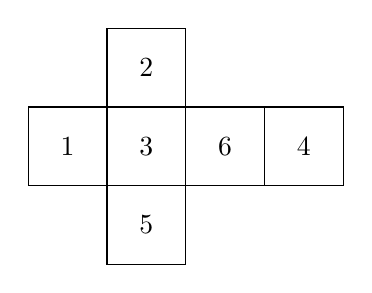
\begin{tikzpicture}
            \node at (0.5,0.5) {1};
            \node at (1.5,1.5) {2};
            \node at (1.5,-0.5) {5};
            \node at (3.5,0.5) {4};
            \node at (1.5,0.5) {3};
            \node at (2.5,0.5) {6};
            \draw (0,0) rectangle (4,1);
            \draw (1,-1) rectangle (2,2);
            \draw (3,0) -- (3,1);
        \end{tikzpicture}
    \end{center}
    \question J'ai lancé un dé 36 fois et j'ai obtenu :
    \begin{center}
        \begin{tabularx}{0.6\linewidth}{|l|C|C|C|C|C|C|}\hline
            Nombre sur le dé & 1 & 2 & 3 & 4 & 5 & 6 \\\hline
            Quantité obtenue & 4 & 6 & 8 & 7 & 5 & 6 \\\hline
        \end{tabularx}
    \end{center}

    Pour savoir si les résultats sont cohérents, il faut se demander si les probabilités obtenues sont proches ou non de la théorie, c'est-à-dire $\frac{1}{6} \approx \num{0.166666}...$
    
\end{questions}

\end{document}